\def\year{2018}\relax
%File: formatting-instruction.tex
\documentclass[letterpaper]{article} %DO NOT CHANGE THIS
\usepackage{aaai18}  %Required
\usepackage{times}  %Required
\usepackage{helvet}  %Required
\usepackage{courier}  %Required
\usepackage{url}  %Required
\usepackage{graphicx}  %Required
\usepackage[UTF8, scheme=plain, punct=plain, zihao=false]{ctex}
\frenchspacing  %Required
\setlength{\pdfpagewidth}{8.5in}  %Required
\setlength{\pdfpageheight}{11in}  %Required
\usepackage{hyperref}

\usepackage{amsmath}


\usepackage[linesnumbered,boxed]{algorithm2e}
%PDF Info Is Required:

\setcounter{secnumdepth}{0}  
\begin{document}
% The file aaai.sty is the style file for AAAI Press 
% proceedings, working notes, and technical reports.
%
\title{Chinese NER with Step-wise Attention}
\author{Xinyue Chen and Fan Xie\\Department of Computer Science and Engineering\\
Shanghai Jiaotong University \\
Minhang, Shanghai, 200240 
\\
kiwisher@sjtu.edu.cn,
fanxie806@gmail.com
}
\maketitle

\begin{abstract}
We investigate a new model for Chinese NER task. Based on the previous state-of-the-art model lattice model for this task, we build a model using attention mechanism that better leverages word-level and character-level information.

\textbf{Our model outperforms lattice model, the previous SOTA} on two datasets without fine tuning of hyper parameters, suggesting its robustness in various corpus.

We borrow much from the lattice model: we also encode a sequence of input characters as well as all potential words that match a lexicon in a sentence. But we further use our step-wise attention instead of the lattice structure to weigh relevance scores of candidate characters and words from a sentence for a more expressive model. We claim that our model helps reduce perplexity and bring a more succinct understanding of corpus. And the results in several corpus proved this assumption.


\end{abstract}

\begin{figure}
\label{fig:lattice}
\centering
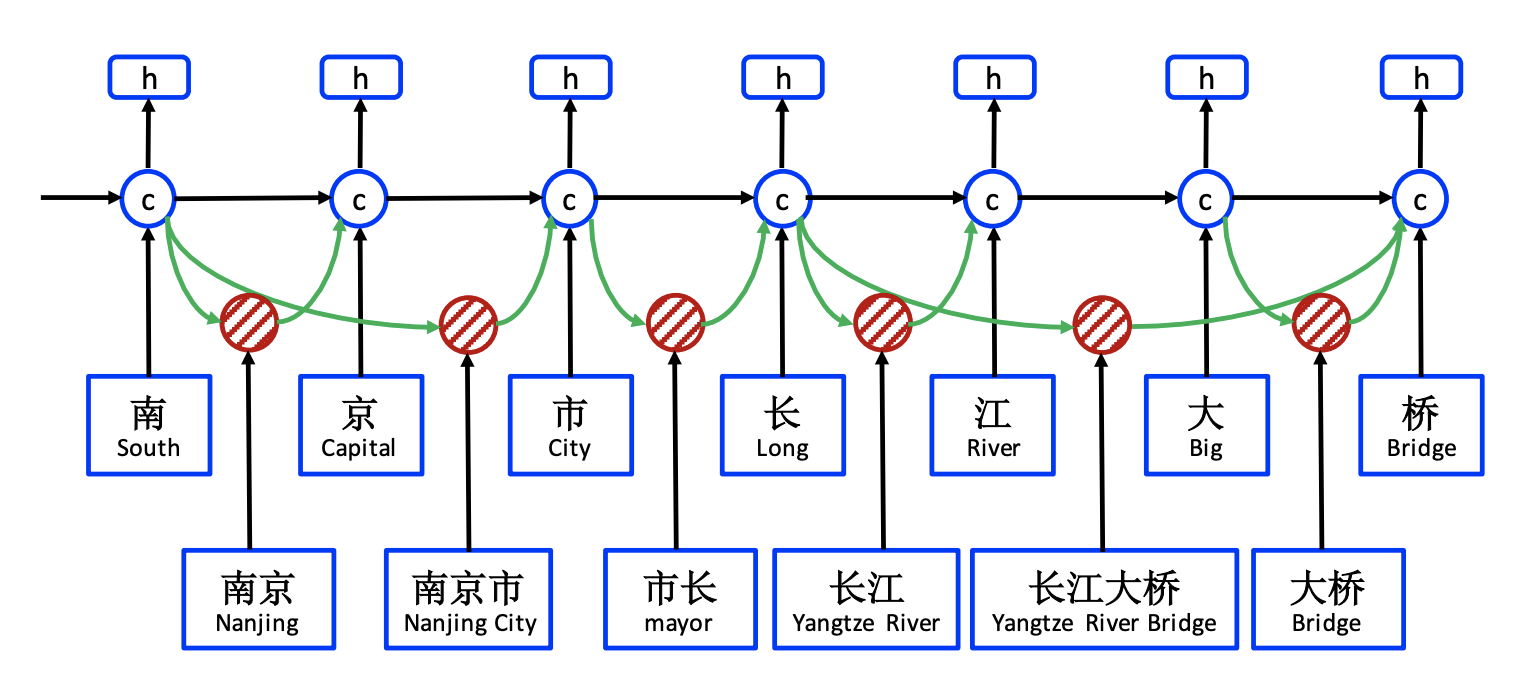
\includegraphics[width=0.5\textwidth]{lattice.png}
\caption{An example for lattice model.}
\end{figure}

\begin{figure*}
\label{fig:our}
\centering
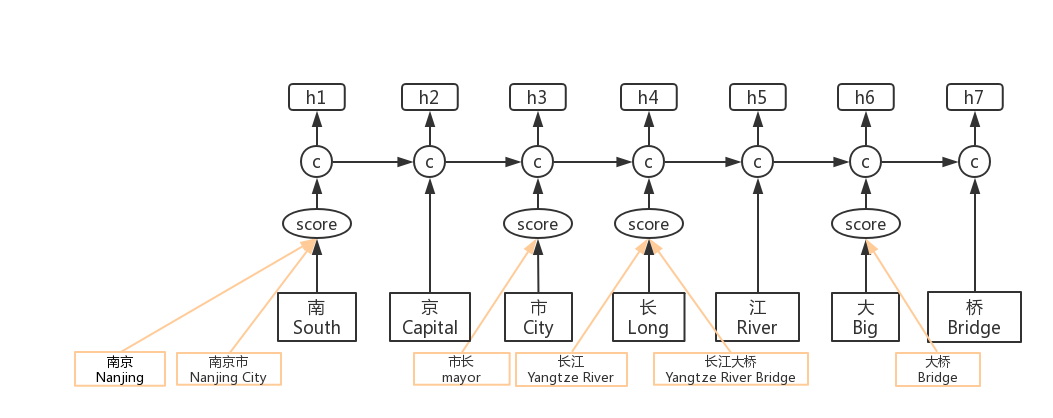
\includegraphics[width=0.7\textwidth]{our.png}
\caption{An example for our model.}
\end{figure*}
\section{1  Introduction}

As a fundamental task in information extraction,
named entity recognition (NER) has received constant research attention over the recent years. The task has traditionally been solved as a sequence labeling problem, where entity boundary and category labels are jointly predicted. The current stateof-the-art for English NER has been achieved by using LSTM-CRF models\cite{lample,ma,chiu,liu} with character information being integrated into word representations.

Chinese NER is correlated with word segmentation. In particular, named entity boundaries are
also word boundaries. One intuitive way of performing Chinese NER is to perform word segmentation first, before applying word sequence labeling. The segmentation 
$\rightarrow$ NER pipeline, however, can suffer the potential issue of error propagation, since NEs are an important source of OOV in segmentation, and incorrectly segmented entity boundaries lead to NER errors. This problem can be severe in the open domain since cross-domain word segmentation remains an unsolved
problem \cite{liu,jiang,huang}. It has been shown that character-based methods outperform word-based methods for Chinese NER.

One drawback of character-based NER, however, is that explicit word and word sequence information is not fully exploited, which can be potentially useful. To address this issue, we integrate latent word information into character-based LSTM-CRF by representing lexicon words from the sentence using step-wise attention mechanism, which is illustrated in \hyperref[sec:our]{this graph}. We align two levels of inputs, word-level and character-level, by matching a sentence with a large automatically-obtained lexicon. As a result, word sequences such as  “长江大桥(Yangtze River Bridge)”, “长江 (Yangtze River)” and “大桥(Bridge)” can be used to disambiguate potential relevant named entities in a context, such as the person name “江大桥 (Daqiao Jiang)”.

Since there are an exponential number of ways for word segmentation, we propose a step-wise attention mechanism for automatically controlling information flow from the beginning of the sentence to the end. As shown in \hyperref[sec:disc]{Section 4}, step-wise attention is used to dynamically route information from different paths to each character. Trained over NER data, LSTM with step-wise attention can learn to find more useful words from context automatically for better NER performance. This model has the advantage of leveraging explicit word information over character sequence labeling without suffering from segmentation error.

We change from lattice to step-wise attention following the pattern that human read sentences-- humans generally make assumptions for the next incoming words and their understandings of the context is constantly changing throughout the whole reading process. 

Results show that our model outperforms the previous state-of-the-art lattice model, giving the best results over two mainstream Chinese NER datasets.




\section{2  Related Work}
Our work is in line with existing methods using neural network for NER. \cite{hammerton} attempted to solve the problem using a unidirectional LSTM, which was among the first neural models for NER. Most recent work leverages an LSTM-CRF architecture. \cite{huang2015} uses hand-crafted spelling features; \cite{ma} and \cite{chiu} use a character CNN to represent spelling characteristics; \cite{lample} use a character LSTM instead. 

Character sequence labeling has been the dominant approach for Chinese NER \cite{dong}. There have been explicit discussions comparing statistical word-based and character-based methods for the task, showing that the latter is empirically a superior choice \cite{li2014}. With proper representation settings, the same conclusion holds for neural NER.

How to better leverage word information for Chinese NER has received continued research attention, where segmentation information has been used as soft features for NER \cite{peng2015,he2017}, and joint segmentation and NER has been investigated using dual decomposition\cite{Xu2014JointSA}, multi-task learning\cite{Peng2016ImprovingNE}. However, the above methods can be affected by segmented training data and segmentation errors.

External sources of information has been leveraged for NER. In particular, lexicon features have been widely used \cite{Collobert2011NaturalLP,huang2015,Luo2015JointER}. \cite{Rei2017SemisupervisedML} uses a word-level language modeling objective to augment NER training, performing multi-task learning over large raw text. \cite{Peters2017SemisupervisedST} pretrain a character language model to enhance word representations. \cite{Yang2017NeuralWS}  exploit cross-domain and cross-lingual knowledgevia multi-task learning. We leverage external data by pretraining word embedding lexicon over large automatically-segmented texts, while semi-supervised techniques such as language modeling are orthogonal to and can also be used for our model.

More recently, \cite{lattice} came with a lattice model, aiming at automatically controlling information flow between word-level and character-level embeddings. However, this model suffers from complexity and confusion entailed by the lattice structure itself. Also, lattice model's fusion of word-level and character-level information is problematic in that the information of a word does not flow into the mainstream (the character-based bi-LSTM) until the timestamp of the last character in the word. 

Based on these observations, we design our model with step-wise attention. Furthermore, we add sentence representation as a global guide in the attention mechanism. 


\section{3 Proposed Model}
There are two primary deficiencies in the lattice model.
\begin{itemize}
\setlength{\itemsep}{12pt}
\item 
\textbf{complexity}

As shown in \hyperref[fig:lattice]{this figure}, the red and blue circles are all LSTM cells, which are costly and time-consuming. Moreover, we claim that this task can be expressed and explained in a more succinct model.

\item \textbf{fusion incoherence}

In the lattice model, the information of a word does not flow into the mainstream (the character-based bi-LSTM) until the timestamp of the last character in the word. For example, in \hyperref[fig:lattice]{this figure}, the information of "长江大桥" (Yangtze River Bridge) flows into the character-level forward LSTM in the last timestamp, bring no direct impact on the labeling of the previous timestamps("长", "江", "大"). 

It is true that correctly defining the label of "桥" helps with the labeling of the previous characters since the labeling of neighboring characters are interrelated. But if the structure becomes more complex, and word-edges become dense in a sentence. Confusion arises inevitably.
\end{itemize}

Therefore, we propose the following model to solve the problem.

\subsection{3.1 Step-wise Attention}
The overall structure of our model with step-wise attention is shown in \hyperref[fig:our]{this figure}, which can be viewed as an extension of the character based model.


Shown in \hyperref[fig:our]{this figure}, the input to the model is a character sequence $c_1, c_2,…, c_m$, together with all character subsequences that match words in a lesion $D$. Using $w_{b,e}^d$ to denote such a subsequence that begins with character index b and ends with character index e, the segment $w_{1,2}^d$ in \hyperref[fig:our]{this figure} is “南京 (Nanjing)” and $w_{7,8}^d$ is “大桥 (Bridge)”. \textbf{Note that from now on, we use $x_{b,e}^{w}$ to denote only these words that not only exists in the sentence as a subsequence, but also is a valid word in our external lexicon.}

This revision of input words is in line with our assumption of the lattice model. We find it more sensible to feed all possible words at the timestamp of its starting character. \textbf{This fusion method is analogous to human reading a paragraph}-- people always make assumptions in the process of reading. And in this reading process, people tend to be more accurate at predicting the next words and gain more understandings of the corpus. So, the model will predict what is the most likely way to segment the part that it is now processing based on the previous hidden state. The prediction is used to score the candidates words (representing possible word segmentation in some sense).


Four types of vectors are involved in the model, namely input vectors, output hidden vectors, cell vectors and gate vectors. As basic components, a character input vector is used to represent each character $c_j$:
\begin{equation}
    x_j^c=e^c(c_j)
\end{equation}
The basic recurrent structure of the model is constructed using a character cell vector and a hidden vector $h_j^c$ on each $c_j$, where $c_j^c$ serves to record recurrent information flow from $c_j$ to the end of the sentence and $h_j^c$ is used for CRF sequence labelling.

The computation of $c_j^c$ now considers lexicon subsequences $w_{b,e}^d$ in the sentence. In particular, each subsequence $w_{b,e}^d$ is represented using
$x_{b,e}^w=e^w(w_{b,e}^d)$
where $e^w$ denotes the word embedding lookup table.
If in a certain sentence, we have $n$ possible words in our lexicon that match with a part of this sentence and start with $c_{b}$, The set of $x_{b,e}^w$ as well as $x_b^c$ will be concatenated together to form a new input $x’_{b,e}^w$. To simplify the notation, we denote $x_{b}^c$ as $x_{b,b}^w$.
\begin{equation}
    x_{b}^w = [x_{b,e_{1}}^w,x_{b,e_{2}}^w,..,x_{b,e_{n}}^w,x_{b,e_{n+1}}^w]
\end{equation}
where $h_{b-1}$ denotes the hidden state of the timestamp just before $b$, and $x_{b,e_{n+1}}^w$ is $x_{b,b}^w$, i.e. the character embedding. For example, the input of the timestamp of "长" is the concatenation of the embeddings of "长", “长江” and "长江大桥".

Then attention is used to compute the score of each $x_{b,e}^w$:
\begin{equation}
    score_{b,e}=h_{b-1}Wx_{b,e}^w
\end{equation}
After scoring the $x’_{b,e}^w$, $x’_{b,e}^w$ becomes:
\begin{equation}
    x’_{b}^w=\sum_{i}score_{b,e_{i}}x’_{b,e_{i}}^w
\end{equation}
In addition, a word cell $c_{b,e}^w$ is used to represent the recurrent state of $x’_{b,e}^w$ from the current character to the end of the sentence. The value of $c_{b,e}^w$ and $h_b^c$ is calculated by:
\begin{equation}
\begin{bmatrix}
i_{b}^w\\
o_{b}^w\\
\tilde{c}_{b}^w
\end{bmatrix}=
\begin{bmatrix}
\sigma\\
\sigma\\
\tanh
\end{bmatrix}
\begin{pmatrix}
\textbf{W}^{w\mathrm{T}}\begin{bmatrix}
x'_{b}^w \\
h_b^c
\end{bmatrix}+\textbf{b}^w
\end{pmatrix}
\end{equation}
where $i_{b,e}^w$ and $o_{b,e}^w$ are a set of input and output gates. In our implementation, the forget gate is simply given as:
\begin{equation}
    f_{b}^w = 1 - i_{b}^w
\end{equation}
We find that this technique helps with the convergence of LSTM models.

\subsection{3.2 Sentence-level Supervision}
As $h_{b-1}$ only contains the information in the previous timestamps (in the perspective of forward LSTM, backward LSTM is similar), we introduce sentence embedding as a global guide to supervise the scoring process in our step-wise attention mechanism.

The intuition is that, even if the information from the previous timestamps might be insufficient, especially in the very first timestamps in a long sentence, with the aid of sentence information, the model will be more capable of comprehending the context and thus predicting the most possible segmentation.

Another thing to consider is how to integrate $h_{b-t}$ with the sentence embedding. We need to integrate these two channels efficiently, without staining their individual semantic information.

We leave a majority of this part to \hyperref[sec:disc]{Section 4} for detailed discussions.

\begin{table*}
    \centering
    \begin{tabular}{|c|c|c|c|c|}
    \hline
    \textbf{Datasets} &\textbf{Models} &\textbf{P} &\textbf{R} &\textbf{F1}\\
    \hline
    \cline{1-5}
    \multirow{OntoNotes}
    &Lattice &76.35 &71.56 &73.88\\
    \cline{2-5}
    &Sentence-level supervision &\textbf{78.05} &\textbf{73.30} &\textbf{73.93}\\
    \hline
    \end{tabular}
    \caption{Main results on OntoNotes}
    \label{tab:onto}
\end{table*}
\newcommand{\tabincell}[2]{\begin{tabular}{@{}#1@{}}#2\end{tabular}}

\begin{table*}
    \centering
    \begin{tabular}{|c|l|c|c|c|}
    \hline
    \textbf{Datasets} &\textbf{Models} &\textbf{P} &\textbf{R} &\textbf{F1}\\
    \hline
    \cline{1-5}
    &Lattice&93.57&92.79&93.18\\
    \cline{2-5}
    &Model 1 &94.62&93.13&93.59\\
    \cline{2-5}
    &\tabincell{r}{Model 2\\\textit{shared}\\\textit{concat}}&\textbf{95.34}&\textbf{93.28}&93.59\\
    \cline{2-5}
    &\tabincell{r}{Model 2\\\textit{shared}\\\textit{mul}}&94.70&92.08&92.74\\
    \cline{2-5}
    \multirow{MSRA}
    &\tabincell{r}{Model 2\\\textit{separate}\\\textit{concat}}&95.03&93.01&93.51\\

    \cline{2-5}
    &\tabincell{r}{Model 2\\\textit{separate}\\\textit{mul}}&95.01&93.02&\textbf{93.67}\\
    \cline{2-5}
    &\tabincell{r}{Model 2\\\textit{separate}\\\textit{concat}\\+$W_{w\rightarrow c}$}&94.33&92.91&92.80\\
    \hline
    \end{tabular}
    \caption{Main results on MSRA}
    \label{tab:msra}
\end{table*}



\section{4 Discussions}
\label{sec:disc}
\subsection{4.1 Sentence Embedding Extraction}

\begin{figure}
\label{fig:multi-head}
\centering
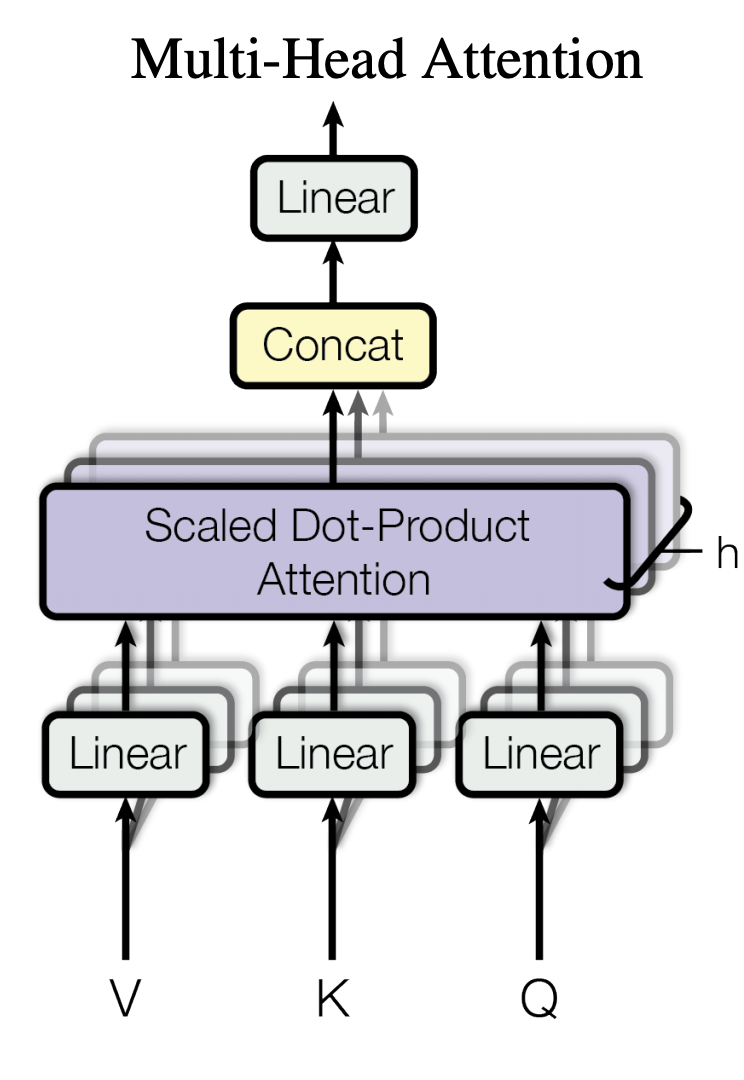
\includegraphics[width=0.2\textwidth]{multi-head.png}
\caption{Multi-head attention.}
\end{figure}
There are generally three methods in our consideration to extract sentence embeddings. We denote sentence embedding as $x^s$

\begin{itemize}
    \item \textbf{Self attention}
    
    Self attention is a special case of multi-head attention \cite{Vaswani2017AttentionIA} where
    \begin{equation}
        Q = K = V
    \end{equation}
    Instead of producing a vector of length $len(e^c)*len(sentence)$, we modify it to produce a fixed-length vector to help it blend in with our model.
    
    The sentence embedding is thus more expressive of the interrelations of characters inside a sentence.
    
    \item \textbf{The last hidden state from LSTM}
    
    This is a more popular way to encode a sentence, which is in line with the encoder-decoder model in NLP tasks. To produce a more expressive representation, we concatenate the last hidden state from both the forward and backward LSTM, so that the embedding will be less biased towards the beginning and end of a sentence.
    
    \item \textbf{The set of hidden states from LSTM}
    
    Instead of using only the last hidden state, we can also utilize all the hidden states from the LSTM.
    
    We can further score the hidden states from a naive LSTM imposing on the sentence, using the hidden state from our step-wise attention model (i.e. $h_{b-1}$) as a judge. Then the weighted average of the elements inside the set of hidden states is integrated with $h_{b-1}$.
    
\end{itemize}


\subsection{4.2 Integration of $h_{b-1}$ and $x^s$}
There are generally three ways to integrate two sources of information.
\begin{itemize}
    \item \textit{element-wise add}
    \item \textit{element-wise multiply}
    \item \textit{concatenate}
\end{itemize}


We believe that \textit{concat} and \textit{mul} operations might be more informative than \texit{add}, because it is too simple to prevent from detailed information losing. 

Though \textit{concat} operation may result in high dimensions, it could keep more information for downstream models to select from. The superiority of \textit{mul} might be due to element-wise product being capable of modeling the interactions and eliminating distribution differences between $h_{b-1}$ and $x^s$, which is intuitively similar to endowing sentence-aware attention over the hidden state. 

So we try both \textit{element-wise multiply} and \textit{concatenate}.

\subsection{4.3 Embedding Space Transformation}

Intuitively, word embeddings and character embeddings are in two different spaces. So it is a natural idea to apply linear transformation before treating them equally in the step-wise attention model.

Therefore, we try to transform word embeddings with matrix multiplication in order to project them into the space of character embeddings. 

It has been proved that orthogonal matrix helps with space transformation. So we try an orthogonal-initialized matrix, $W_{w\rightarrow c}$. But experiments show that this method hurt our model's performance. Possible reasons are:
\begin{itemize}
    \item \textbf{The embedding vectors are fine-tuned during training.}
    
    Since embeddings are to be back-proped. The gap between different spaces might be bring to a semantic harmony.
    
    \item \textbf{Redundancy}
    
    Adding an additional parameter $W_{w\rightarrow c}$ may slow down the convergence of model.
\end{itemize}




The same as model mentioned before, scoring function is used in the model. The integrated hidden state scores the $x'$.


\section{2 Experiments}

We carry out an extensive set of experiments to investigate the effectiveness of our model in two named datasets for Chinese NER.

\subsection{4.1 Experiment Settings}
We borrow much of the settings from \cite{lattice}, but we achieve higher performance with our step-wise attention without tuning hyper parameters.

\textbf{Dataset} 

We used two datasets in this experiment: OntoNotes 4 and MSRA. 

\textbf{Embeddings} 

Word embeddings is pretrained by word2vec over automatically segmented Chinese Giga-Word, obtaining 704.4k words in a final lexicon. In particular, the number of single-character, two- character and three-character words are 5.7k, 291.5k, 278.1k, respectively. Word embeddings are fine-tuned during NER training. Character and character bigram embeddings are pretrained on Chinese Giga-Word using word2vec and fine-tuned at model training.


\textbf{Result Notations}

Here we clarify our notations used for reporting our experiment results.

\begin{itemize}
    \item \textbf{Model 1}: Our step-wise attention model without sentence-level supervision
    
    \item \textbf{Model 2}: Our step-wise attention model with sentence-level supervision
    \item \textbf{shared / separate}: Whether a sentence embedding is shared among both directions of LSTM or for each LSTM use a separate sentence embedding. 
    
    Due to time limit, we implement sentence embedding extraction via self attention.
    
    \item \textbf{w2c / $W_{w\rightarrow c}$}: Indicate whether a model uses word-to-character embedding space transformation.
\end{itemize}

\subsection{4.2 Final Results}
We fail to reproduce the results from \cite{lattice} even with their own code. So we only compare our model with the lattice one in the form of tables, i.e. best results.


\textbf{MSRA} 

\begin{figure}
\label{fig:msra}
\centering
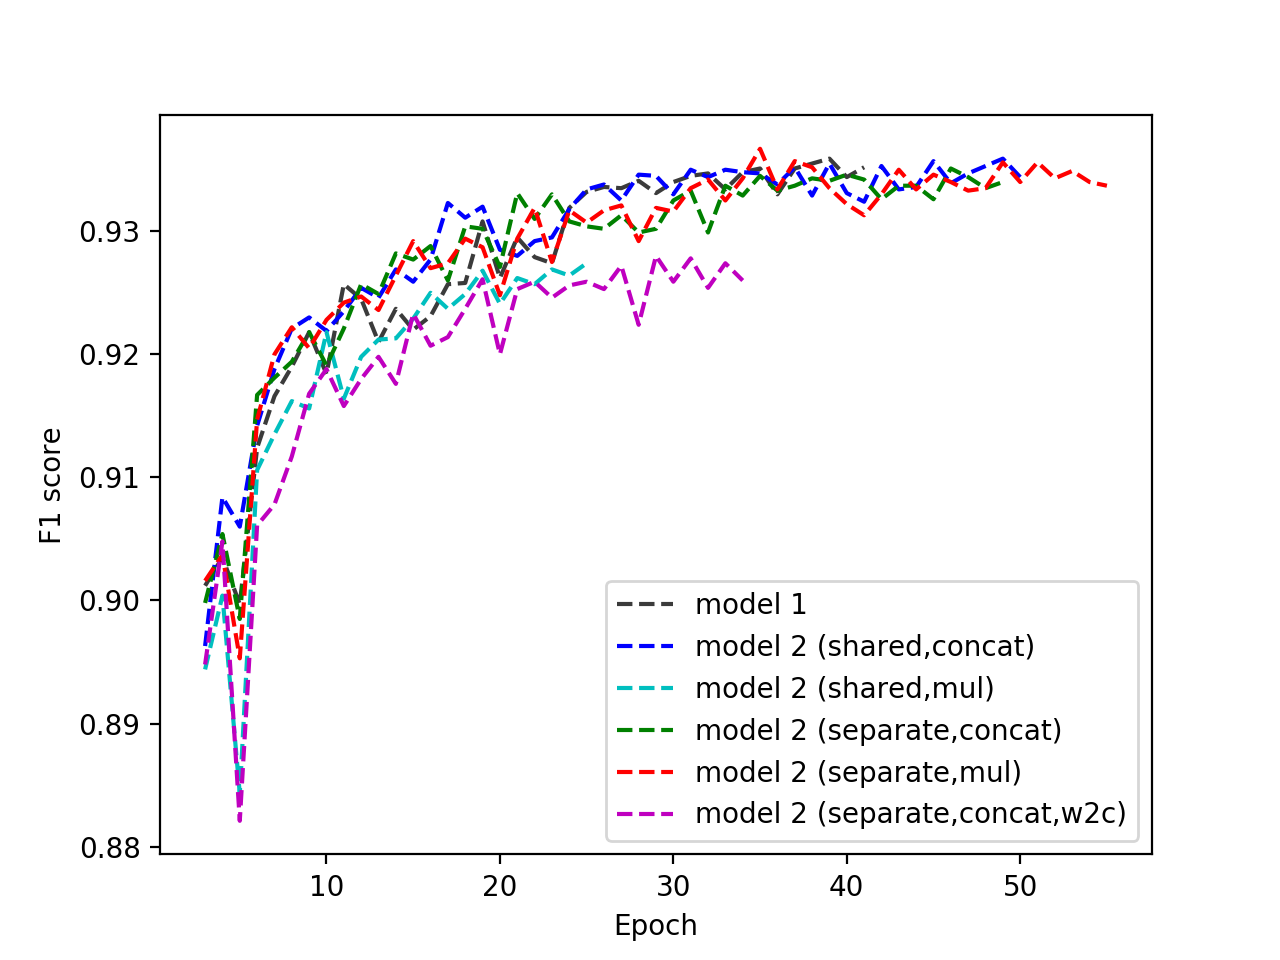
\includegraphics[width=0.5\textwidth]{MSRA.PNG}
\caption{F1 against training iteration number on MSRA.}
\end{figure}

The results of MSRA are shown in \hyperref[tab:msra]{this table}. Among all the tested models, the values of precision and recall of step-wise attention model with concatenation are significantly higher than lattice model. Sentence-level supervision model with multiplication and without $W_{w\rightarrow c}$ has the highest F1 value. And model with $W_{w\rightarrow c}$ gives a F1-score of 92.38\% doesn't have a better performance than the same basic model without $W_{w\rightarrow c}$. This fact tells us that the existence of embedding space transformation does not help.

\hyperref[fig:msra]{This figure} shows the F1-score of models on MSRA dataset against the number of training iterations. As shown in the figure, the value of model 1 with \textit{mult} and no w2c and the value of model 2 with w2c and concatenation are generally smaller than the other models.

From \hypertarget{tab:msra}{Table 2}, we can see that most of our proposed models significantly outperforms the lattice one.

\textbf{OntoNotes} \hyperref[tab:onto]{This table} shows the results on OntoNotes dataset. The P, R, and F1 values of sentence-level supervision model are higher than lattice model. Due to time limit, we only implement our model 2 with separate sentence embedding on this dataset. And it also achieves better performance than the lattice model. Therefore, we can draw a conclusion that our step-wise attention model with sentence-level supervision outperforms lattice model. 







\bigskip

\section{Acknowledgements}
We thank Professor Jiang for presenting us with this opportunity and guiding us in digging the specific problem. Also, we would like to express our gratitude for the author of \cite{lattice}, Jie Yang, who kindly exchanges ideas with us.



\bibliographystyle{aaai} 
\bibliography{ref}

\end{document}
